\chapter{Estado da Arte}\label{arte}

%Introdução, Motivação e Objetivo
\section{Introdução}\label{arte:intro}

Astrônomos atualizam suas descobertas numa base de dados disponíveis para outros utilizarem; as ciências biológicas agora têm tradição 
em depositar seus avanços científicos em repositórios públicos; redes sociais estão focadas na Web: Facebook, LinkedIn, Microsoft, 
Tweeter e Yahoo sobrevivem coletando informações e repassando-as às empresas de telemarketing, empresas de comércio eletrônico como 
Amazon.com, Submarino.com.br, Americanas.com, MagazineLuíza.com.br, utilizam essas informações para vender mais e melhor. 
Por outro lado, artigos científicos dos mais variados assuntos e das mais variadas áreas alimentam todos os dias, com milhões de 
informações, os \textit{Data Centers}. Esse é o paradigma do \textit{Big Data}.

Nesse estudo, para fazer frente ao paradigma acima aludido e extrair informações com eficácia, 
foi proposto o desenvolvimento de um mapeamento sistemático.

\section*{ Mapeamento sistemático}

Foi desenvolvido a priori um mapeamento sistemático das mais diversas tecnologias empregadas no ``Big Data'' e seus paradigmas para extrair informações e conhecimentos, 
analisando as técnicas de Inteligência Artificial mais empregadas nesse campo científico de exploração.
A posteriori; propor uma solução à logística de cargas aplicada à realidade brasileira, antecipando os problemas que possam surgir no traçado de rotas determinísticas. 

O mapeamento sistemático foi definido em etapas da seguinte forma:

\begin{enumerate}
 \item[A.] Coleta dos dados;
 \item[B.] Seleção dos artigos; 
 \item[C.] Escolha dos Filtros;
 \item[D.] Leitura dos artigos.
\end{enumerate}


\subsection{Detalhamento das etapas}

\begin{enumerate}
 \item[A.] Coleta dos dados\\
    Para coletar os dados foram escolhidas seis palavras-chave com relevância para o tema, a saber:
    \begin{itemize}
      \item “Data Mining and Swarm Intelligence”
      \item “Data Mining Big Data”
      \item “Data Mining Swarm Robotics”
      \item “Hadoop Map Reduce in Big Data”    
      \item "Machine Learning"
      \item “Map Reduce Big Data”
    \end{itemize}


    A partir das palavras-chave foram criadas planilhas, sendo cada aba representada por uma palavra-chave. 
    Incluiu-se no mínimo 30 artigos para cada aba da planilha, totalizando 316 artigos.
    Pretendeu-se, com essa técnica, construir rapidamente gráficos das mais diferentes matizes, tais como:
    \begin{itemize}
      \item Base pesquisada;
      \item Data da publicação;
      \item Parecer (Aceito ou rejeitado);
      \item Título do artigo;
      \item País de origem.
    \end{itemize}

    A ferramenta utilizada para obter os dados referentes às palavras-chave (referência bibliográfica) foi o programa Mendeley, especializado 
    em extrair dados de arquivos como artigos, dissertações e teses.
    A figura 2.1 a seguir mostra como a Planilha-Survey se apresenta:
  
    \begin{figure}[!ht]
      \centering %\centering % para centralizarmos a figura
      \caption{Planilha Survey}
      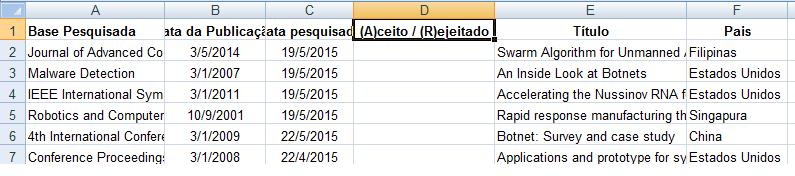
\includegraphics[width=110mm, height=40mm]{Figuras/BigData/PlanilhaSrvey.jpg}
    \end{figure}
  
 \item[B.] Seleção dos artigos\\
    A seleção dos artigos foi primeiramente escolhida pelas mais recentes publicações dos últimos 5 anos, expecificamente entre 2010 e 2015. 
    O segundo critério de seleção foi pelo órgão publicizador, considerando os mais conhecidos, tais como IEEE, Elsevier, Springer, bem como os jornais a eles pertencentes. 
    Outras fontes foram tabém consideradas, como universidades e seminários mais conhecidos na área.
    Outro critério considerado foi a seleção de no mínimo de 30 (trinta artigos) por palavra-chave.
    Dessa forma, procuramos aproximar os dados coletados da distribuição normal padrão, que por razões evidentes está amplamente
    tabelada e é suprida por quase todos os softwares para construtores de gráficos.\\

\pagebreak
    
 \item[C.] Critérios de Inclusão/Exclusão \\
    O critério de inclusão e exclusão foi baseado na leitura dos ``abstracts'' dos artigos. 
    Devido ao fato de algumas palavras-chave estarem muito em evidência, as mesmas são citadas em diversos artigos sem referência para tema,
    não sendo relevante para a pesquisa. Dessa forma foi criada uma pasta chamada ``Rejeitados'' para onde foram movidos esses artigos.
    Outro critério de exclusão foi data anterior a 2010, com exceção dos artigos clássicos da área.\\

 \item[D.] Leitura dos artigos \\
    A leitura dos artigos iniciou-se após a etapa de Inclusão/Exclusão.
    Até o momemto foram lidos 72 artigos de um total de aproximadamente 240 artigos.
    Segue uma tabela com as datas do plano de execução.
    
    \begin{table}[htbp]
      \scriptsize
      \centering
      \caption{Datas do Survey}
	\begin{tabular}{l|c|c|c}
	\hline
	\textbf{Data/2015} & \textbf{(A) Coleta} & (B) \textbf{Seleção} & \textbf{(C) Filtros} \\
	\hline
	Abril a Junho & x & --- & --- \\ \hline
	Junho e Julho & -- & x & x \\ \hline
	Agosto & -- & -- & x \\ \hline
	\end{tabular}
    \end{table}
  
 \end{enumerate}



\section*{ Big data}

"Em 2010 empresas e usuários armazenaram mais de 13 exabytes de novos dados" \cite{bigdataQualquerUm}.

O \textit{Big Data} pode ser definido como um paradigma dos 3 V’s, descrito como: 

%Tabela 4
\begin{table}[htbp]
 \begin{itemize}
   \item Volume de dados;
   \item Velocidade para acessar esses dados;
   \item Variedade de informações;
 \end{itemize}
\end{table}

  
Dentre as mais diversas técnicas encontradas para acessar dados no \textit{Big Data} destacamos o Map Reduce, da ``framework'' Hadoop, por ser de livre uso (freeware) e 
por ser tolerante a falhas, sendo de fácil implementação e de baixo custo para a maioria das pequenas empresas e pesquisadores.
A tecnologia congênere, desenvolvida pelo Google, (``Google File System'') merece ser destacada. 
Não é tarefa trivial inferir e desenvolver novas ferramentas para o \textit{Big Data}, dada a dimensionalidade do problema, conforme destacado na tabela a seguir:


%tabela 5
\begin{table}[!ht]
\centering
\caption{Volume de dados no mundo}
\vspace{1mm}
\begin{tabular}{l|c|c|c}
\hline
\textbf{Ano} & \textbf{Qtd} & \textbf{Unidade} & \textbf{Múltiplo}\\
\hline
2000 & 800 & terabytes – TB & $10^{12}$\\
2006 & 160 & petabytes – PB & $10^{15}$\\
2009 & 500 & exabytes – EB & $10^{18}$ \\
2012 & 2,7 & zettabytes – ZB & $10^{21}$\\
2020 & 35 & yottabytes – YB & $10^{24}$\\
\end{tabular}
\end{table}

\pagebreak

Com a chegada da Internet das Coisas, conhecida como ``A terceira onda da Internet'', os dados irão aumentar exponencialmente. Por exemplo, 
os produtos nas gôndolas do supermercado, com um novo tipo de etiqueta se conectam a uma leitora de radio frequência a alguns metros de distância, 
contabilizando o total do estoque em segundos; o consumidor leva seus produtos escolhidos ao caixa desse supermercado, pagando a conta sem precisar retirar qualquer 
produto do carrinho. Ao introduzir esses produtos na geladeira, será possível saber quando expirará a data de validade de determinados produtos, sem 
precisar abri-lo, e quando acabarem esses produtos, a própria geladeira informará ao supermercado a falta deles, reservando o próximo rol de compras. 
Assim poderá se dar essa onda de coisas conectadas, que fará com que os dados sofram emplosão combinatória de informações, multiplicando exponencialmente as dimensões do 
\textit{Big Data}.

As redes sociais são um arcabouço de informações sobre todo tipo de assunto vivenciado no cotidiano das pessoas, inclusive situações que dizem respeito ao nosso ambiente de pesquisa.
O cenário abaixo, encontrado numa rede social, exemplifica a sequência de informações retiradas do Twitter, um microblog onde os usuários escrevem num pequeno espaço (cerca de 140 caracteres), 
os mais diversos assuntos, e os usuários conectam por uma multiplicidade de dispositivos: computadores, tablets e celulares, formando uma grande rede social mundial. 
A ideia inicial do Twitter, segundo seus fundadores, era que essa rede se comportasse como um ``SMS da Internet'' \cite{Twitter2015}. 
As informações são enviadas aos usuários, conhecidas como twittes, em tempo real e também enviadas aos usuários seguidores que tenham assinado para recebê-las.

%\pagebreak

A seguir pode-se verificar uma sequência de twittes da Polícia Rodoviária Federal de Santa Catarina:

\begin{figure}[ht]
\subfigure{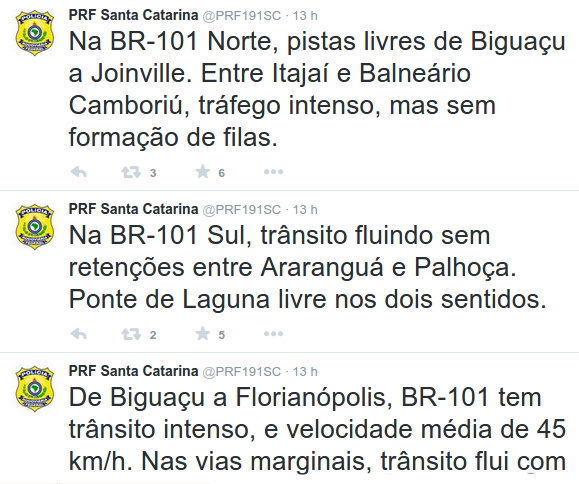
\includegraphics[width=60mm, height=48mm]{Figuras/BigData/twittePRF.png}}
\quad \quad \quad \quad
\subfigure{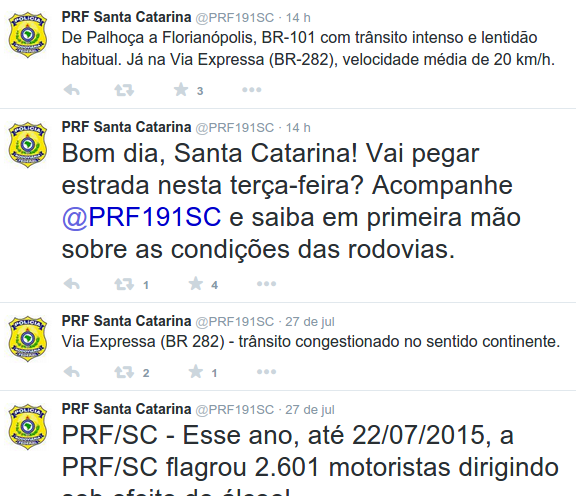
\includegraphics[width=60mm, height=48mm]{Figuras/BigData/twittePRF2.png}}
\end{figure}

A Polícia Rodoviária Federal de Santa Catarina, disponibilizou às 13h através do canal @PRF191SC, informações relevantes sobre o trânsito naquela localidade, 
num espaço temporal variado, por exemplo: entre Itajaí e Balneário Camboriú o transito está intenso. Isso sugere que a frota de caminhões deva ter uma
rota alternativa caso a situação persista por muito tempo. No primeiro twitte da segunda coluna, é informado em Via Expressa (BR 282) que o trânsito está lento com 
velocidade de 20km/h (praticamente congestionado). Essa informação sugere que deve ser pensada uma rota alternativa, caso o congestionamento persista por muito tempo.

Outra rede social conhecida pelos condutores de veículos é o Waze. O Waze é um aplicativo de navegação para o trânsito, funciona em aparelhos celulares e tablets. 
Os utilizadores desse aplicativo são conhecidos como wazers e compartilham informações sobre o trânsito, em tempo real. Toda via, as informações somente estão disponíveis 
no momento em que são postadas pelos utilizadores, por um período de tempo pequeno. Caso não haja usuários trafegando pelas vias ou caso os mesmos não tenham disponibilidade 
em postar informações, não há o que se compartilhar.
Outro problema levantado com o waze é que, caso não haja conexão à Internet não há como acessar os dados dos 'wazers', para navegação.

Além dos dados que chegam ao \textit{Big Data} através das redes sociais, as grandes cidades têm disponíveis câmeras de monitoramento do trânsito nos semáforos ou próximas a eles; 
algumas com cobertura por canais de televisão bem como câmaras de segurança próximos às rodovias, coletando informações em tempo real. 
Os dados desses dispositivos são gravados, sendo conhecidos como \textit{stream} de dados. 
Esses \textit{streams} podem ser disponibilizados na Internet, em sítios eletrônicos especialmente construídos para isso, como o http://vejoaovivo.com.br dentre outros.

Os dados disponibilizados pelos diversos meios de comunicação não estão em formato que possam ser utilizados imediatamente, precisando antes serem processados. 
Tais dados não processados são conhecidos como ``dados frios''. O processo de tratar as informações, retirando-lhes o ``lixo'' e transformando dados ``frios'' em dados 
``quentes'', é um processo que tem um custo temporal elevado, devido ao volume dos dados.

%\pagebreak

Para trabalhar com os dados do \textit{Big Data} a empresa Google (Google Inc.) criou uma arquitetura para computadores trabalharem remotamente em conjunto, formando um 
\textit{cluster}. Essa arquitetura reestrutura o sistema de arquivos, o \textit{filesystem} \footnote{\textit{Filesystem} referem-se à forma como os dados são armazenados, 
organizados e acessados, pelo sistema operacional, em cada partição no disco (ou no disco rígido inteiro)} \cite{Filesystem} e os diretórios dos computadores com certas 
características, conhecido como HaDoop FileSystem (HDFS). 
O Hadoop é uma implementação em código aberto da técnica Map-Reduce.


\subsection{Map Reduce - Big Data}\label{arte:palavraChave:MapReduceBigData}


O Map-Reduce é uma técnica conhecida desde a linguagem Lisp, impĺementado sob uma arquitetura HDFS (ou GFS) que permite mapear os \textit{clusters} e reduzir a quantidade de
 informação conforme um par de informações <chave:valor>.
A imagem a seguir exemplifica essa técnica:

\begin{figure}[ht]
\centering
\caption{Técnica Map-Reduce}
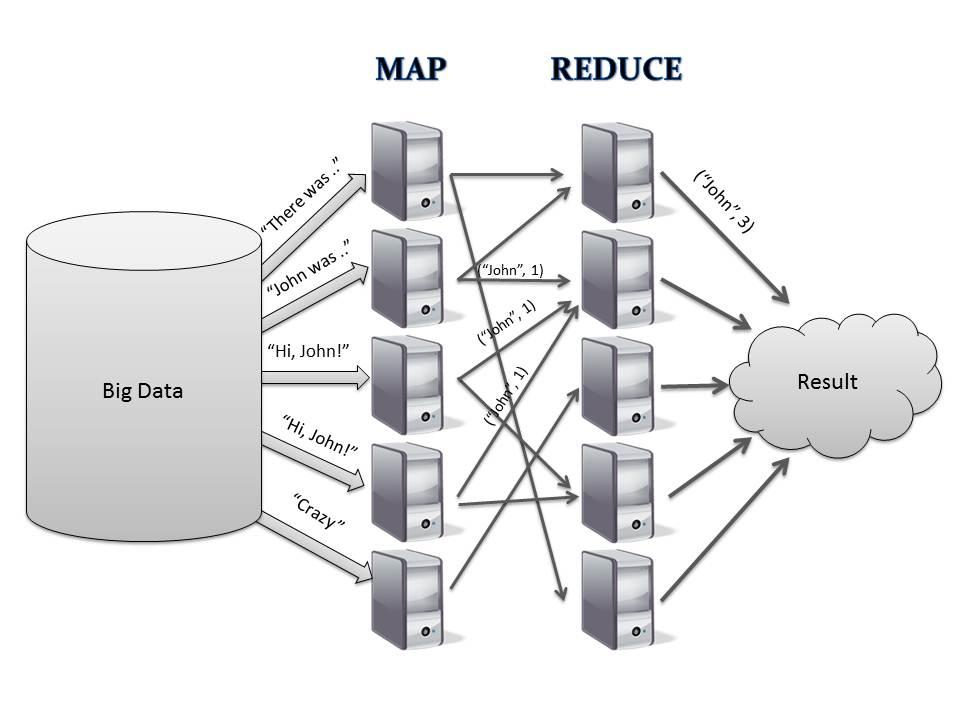
\includegraphics[width=80mm, height=60mm]{Figuras/BigData/MapReduce.jpg}
\end{figure}

Map-Reduce; modelo de computação paralela para ser utilizado na Internet foi proposto pelo Google \cite{Dean2008}.


\subsection{Hadoop - Map-Reduce - Big Data}\label{arte:palavraChave:HadoopMapReduce}

O Hadoop é uma arquitetura de milhares de computadores interligados paralelamente e espalhados pela Intenet formando \textit{cluster}.
Esse \textit{cluster} tem a característica de grande escalabilidade, em torno de 3 000 computadores, dependendo da construção e tolerância a falhas. 
Quando um computador do \textit{cluster} fica inoperante ou ``cai'', os dados são salvos em outro computador. 

A estrutura de diretórios do Hadoop foi especialmente construída para lidar com as características descritas anteriormente, devido ao baixo custo de implementação e 
por ser uma tecnologia aberta (\textit{Open Source}), tendo sido desenvolvida por programadores do mundo todo. A versão Hadoop da empresa Google é o Google Filesystem (GFS).

Os \textit{clusters} de computadores, aplicando a técnica de programação Map-Reduce estão preparados para extrair dados do \textit{Big Data}, contudo até que esses dados 
estejam prontos para mineração eles devem seguir um fluxo de operações para transformá-los em dados relevantes (quentes).
O fluxo seguido pela informação, desde o local onde é produzida até o momento em que possa ser utilizada está dividido em etapas na imagem a seguir:

\begin{figure}[!ht]
\centering
\caption{Big Data e Arquitetura Hadoop}
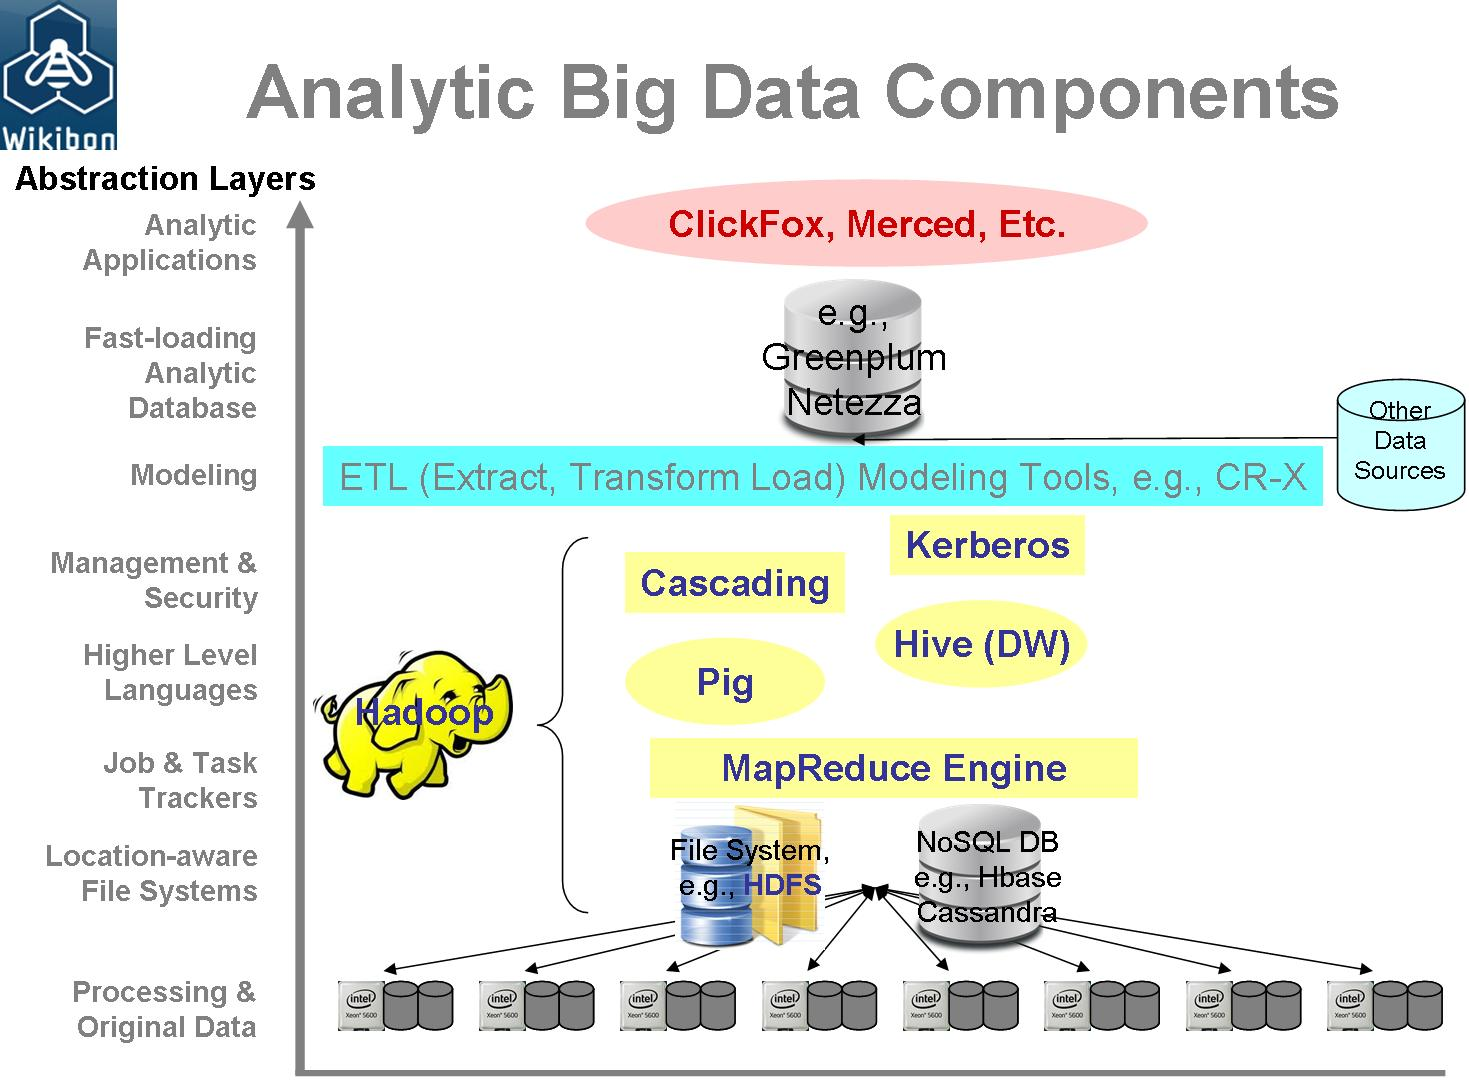
\includegraphics[width=90mm, height=70mm]{Figuras/BigData/BigDataComponents.jpg}\\
\tiny Fonte: Wikibon -- 2015
\end{figure}

A camada mais baixa da imagem, onde se lê \textit{Processing \& Original Data} é a origem do \textit{Big Data}, onde estão os dados ``frios''. 
Entre as camadas \textit{Location-aware File Systems} e \textit{Management \& Security} a informação é mapeada no Hadoop e em seguida a técnica Map-Reduce é empregda, reduzindo
o volume dos dados. Em Hive (Datawarehouse - DW) é possível armazenar os dados, esses dados são considerados ``quentes''. Em \textit{Modeling} ocorre o que se chama de 
\textit{Extract, Transform and Load} (ETL) ou Extração, Transformação e Carga, que é onde se inicia a mineração de dados.
Mais adiante aprofundaremos a discussão sobre Mineração de dados.

\pagebreak


\section{Data Mining}

Técnicas de mineração de dados trabalham com dados estruturados, preenchidos em sua totalidade (sem \textit{missing data}), para poder extrair informações relevantes.
Um dos maiores problemas na extração de informações é que os dados não estão estruturados, ou não estão no grão adequado, ou ainda faltam dados (``missing data'' -- dados ausentes). 
Para contornar o problema de dados ausentes existem várias técnicas, como preenchimento dos dados através de técnicas de inteligência artificial.

O caminho da extração dos dados até sua mineração e, por fim, extração de conhecimento é longa.
Na figura a seguir temos um exemplo desse caminho:

\begin{figure}[!ht]
\centering
\caption{Minerando dados no Big Data}
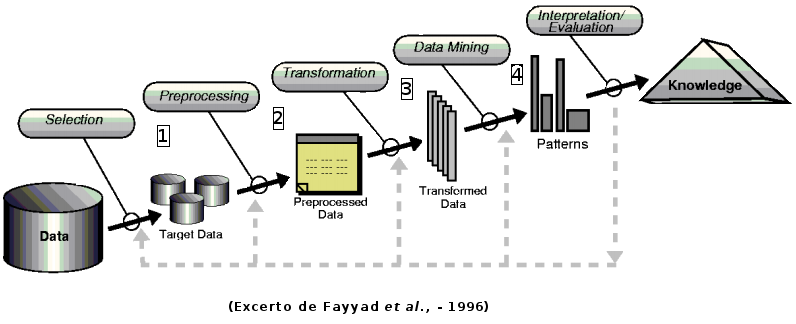
\includegraphics[width=140mm, height=90mm]{Figuras/BigData/FayyadSemFundo.png}
\end{figure}


O Big data está representado na figura onde se lê ``Data'' e está repleto de \textit{missing data} e/ou dados inconsistentes, conhecidos como dados não estruturados. 
O balão onde se lê ``Selection'' representa a coleta das informações ou a seleção dos dados no \textit{Big Data}.
Em nossa pesquisa esses dados são provenientes das mais diversas fontes, tais como, redes sociais, câmaras de trânsito, informações de satélites meteorológicos e outras fontes.

Armazenar qualquer quantidade de dados nessa etapa pode ser um grande problema, devido à sua extensão, porém os dados relevantes podem ser armazenados em ``Target Data'' 
com a tecnologia Hadoop, utilizando as técnicas de ``Map'' e ``Reduce'' para criar \textit{cluster} de informações e ler os fluxos de dados (stream data). Algumas técnicas de 
IA podem ser aplicadas nessa etapa como, ``Data Mininng Swarm Robotics'' através de Botnets \footnote{Botnet é citado no sentido da coleta de informações} ou ``Swarm Intelligence''. 

No balão ``Preprocessing'' os dados não-estruturados são tratados, por exemplo, retirando os \textit{missing data}. 
Para estruturar as informações é preciso utilizar técnicas linguísticas, uma vez que existe lógica entre eles \cite{Aranha2006}.
Esses dados normalmente são coletados por técnicas de Mineração de Textos, também conhecidas como Mineração de Dados em Textos, técnicas de IA como ``Machine Learning'' 
têm sido muito utlizadas. Em ``Transformation'' os dados foram em estruturados, podendo ser armazenados em Bancos de Dados, conhecidos como Datawarehouse, por exemplo o Hive. 

O processo de Mineração dos dados começa no balão ``Data Mining'', onde são aplicadas as técnicas de IA conhecidas como classificadores, para extração de padrões, tais como: 
``Decision Tree'' (Árvore de decisão), ``Artificial Neural Network'' (Redes neurais artificiais), ``Logistic Regression'' (Regressão Logística) e ``Deep Learning''.
Algumas técnicas de mineração de dados são fortemente influenciadas pelas informações na entrada (input), como as Árvores de decisão \cite{DecisionTree}. 
As Redes Neurais, dependendo da quantidade de variáveis de entrada, paderão ter milhares de neurônios na camada intermediária, o que inviabilizaria essa metaheurística 
\footnote{Metaheurística são heurísticas aplicadas em problemas onde os custos computacionais não são tratáveis em tempo polionomial, devido às explosões combinatórias geradas
pelo grande número de tentativas. Metaheurísticas bioinspiradas metaforizam o comportamento de animais sociais, tais como formigas, pássaros, peixes e outros}.

Todas essas etapas descritas na figura são recorrentes, como indicam as setas pontilhadas que retornam aos passos anteriores.
Utilizar técnicas de mineração de dados, além de extrair dados, extrai conhecimento, com isso pode-se predizer os resultados futuros na saída do modelo, 
quando determinados dados ocorrem na entrada \cite{Amin2015a}, essa técnica de extração de conhecimento chama-se \textit{Knowledge Discovery Databases} (KDD).


\subsection{Data Mining - Big Data}\label{arte:palavraChave:DataMiningBigData}

Minerar dados no \textit{Big data} não é uma tarefa atômica, devendo ser divida em várias etapas, com processos específicos em cada uma delas, como descrito anteriormente. 
Extrair conhecimento dos dados não processados não faz sentido, tratá-los apenas ``per si'' exige muito trabalho de IA, como Mineração de dados em textos. 
A Mineração em textos é inspirada em técnicas de ``Machine Learning'' \cite{Aranha2006}. 
Contudo analisar textos é basicamente entender o significado do texto, baseado em regras de associação lógica.
O mapa mental a seguir mostra um modelo de análise de texto feito por seres humanos.

\begin{figure}[htpb]
\centering
\caption{Mapa mental da Mineração em textos}
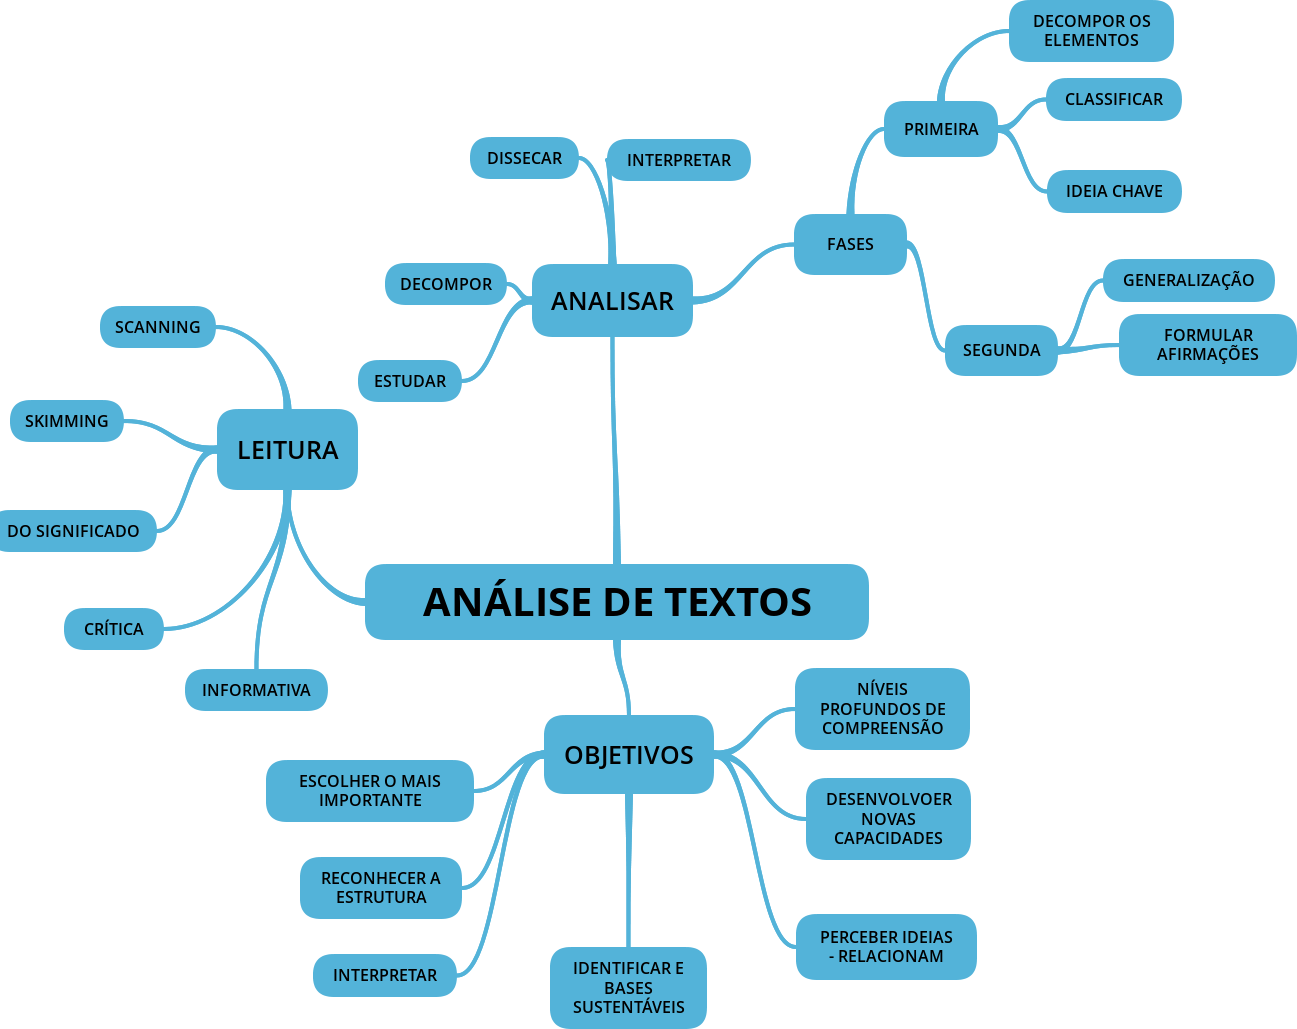
\includegraphics[width=120mm, height=60mm]{Figuras/BigData/Analise_Textos.png}
\end{figure}


O processo de mineração ``CRoss Indrustry Standard Process for Data Mining'' (CRISP-DM) \cite{Crisp2000} descreve como os especialistas em mineração de dados aplicam as técnicas em lide.
O CRISP-DM é um processo recursivo, onde cada etapa deve ser revista até quando o modelo apresentar os resultados satisfatórios, preliminarmente definidos.
O Analista de Dados ou o Cientista de Dados é o profissional que acompanha e executa o modelo de predição, como exemplificado na figura a seguir:

\begin{figure}[!ht]
\centering
\caption{O padrão CRISP-DM}
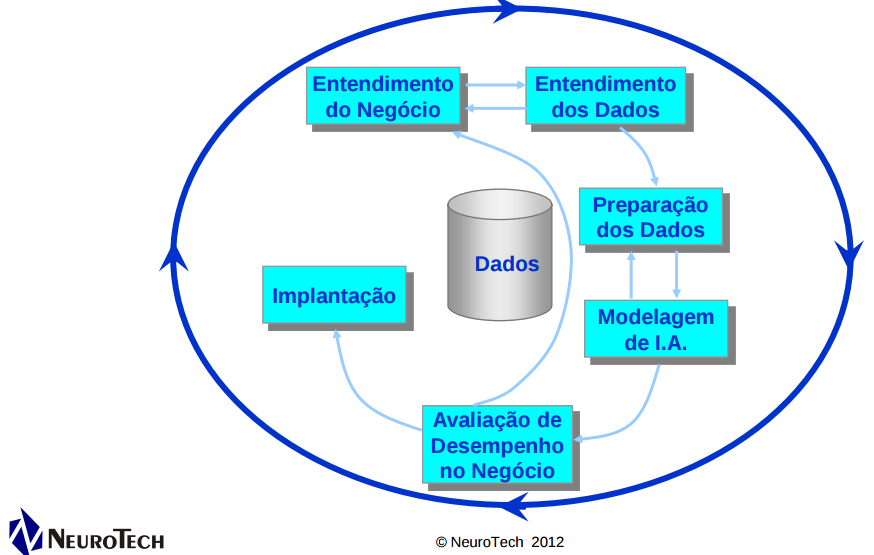
\includegraphics[width=80mm, height=60mm]{Figuras/BigData/CrispDM.png}
\end{figure}

O \textbf{Entendimento do negócio} é uma fase crucial da mineração, um especialista (ou muitos) deve ser consultado. O analista de dados consegue fazer re-uso de conhecimento lendo periódicos e artigos, 
mas a experiência de um profissional da área é condição ``sine qua non'' nessa fase.
Após a primeira fase, o analista de dados à fase do \textbf{Entendimento dos dados}. Nessa fase o analista ``olha'' para os dados com a acurácia de um especialista, 
procurando identificar qualidade nos dados. Dados ausentes são comuns em bases de dados não estruturadas, os ``missing data'' são sempre um problema a ser considerado, 
pois seu tratamento pode consumir muito tempo do analista de dados. 
A fase da \textbf{Preparação dos dados}, cobre a construção final do conjunto de dados. Preparar os dados significa criar e selecionar atributos, criar tabelas ou planilhas e registros dos dados.

Na fase de \textbf{Modelagem de I.A.} a tecnologia deve ser escolhida com critério baseado em experiência do analista de dados. 
Em sistemas de suporte à decisão, uma tecnologia inadequada pode levar a decisões imprecisas. É comum retornar às fases anteriores para adequar a técnica aos dados. 
Um modelo de regressão logística para problemas binários, redes neurais para problemas de classificação e assim por diante.

Na fase da \textbf{Avaliação de desempenho} um ou muitos modelos devem ter sido construídos e testados, apresentando alta qualidade da perspectiva da ánalise dos dados.
Criar um modelo geralmente não é o fim do processo, contudo é um modelo de entendimento do negócio. 
Até que se obtenha as respostas satisfatórias, o modelo deverá ser refeito várias vezes até sua \textbf{Implantação}. 
A próxima figura descreve o domínio das técnicas aplicadas à mineração de dados:

\begin{figure}[!ht]
\centering
\caption{Domínio das técnicas aplicadas a mineração de dados}
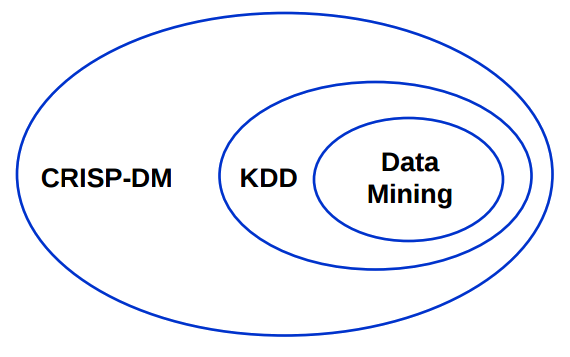
\includegraphics[width=65mm, height=28mm]{Figuras/BigData/RelacaoCrispKddDm.png}\\
\tiny Fonte: Neurotech -- 2012
\end{figure}


Quando são desenvolvidos sistemas de predição e ánalise de diagnóstico, há que se avaliar o desempenho e a qualidade dos resultados encontrados.
Um método gráfico eficiente para detecção e avaliação da qualidade de sinais, conhecido como \textit{Receiver Operating Characteristic} -- ROC, ou curva ROC \cite{ROC},
foi criado e desenvolvido na década de 50 do século passado, para avaliar a qualidade da transmissão de sinais em um canal com ruído.
Recentemente a curva ROC tem sido adotada em Mineração de dados e Aprendizagem de Máquina \cite{MD_AM}, em sistemas de suporte à decisão na medicina, para analisar a qualidade da detecção 
de um determinado teste bioquímico, na psicologia para detecção de estímulos \cite{Discriminativo} em pacientes, e na radiologia para classificação de imagens.

Essas métricas são amplamente utilizadas na classificação binária de resultados contínuos. Para isso ser construido, a Matriz de Contingência classifica as probabilidades como:
verdadeiro positivo, falso positivo, falso negativo e verdadeiro negativo, respectivamente \textit{True Positive -- TP, False Positive -- FP, False Negative -- FN e True Negative -- TN },
também conhecida como matriz de confusão, descrita na tabela a seguir:

%tabela 5
\begin{table}[ht]
\centering
\caption{Matriz de Confusão}
\vspace{1mm}
\begin{tabular}{l|c|c}
\hline
\textbf{} & \textbf{Predito} & \textbf{}\\
\hline
\textbf{Real}  & TP   FN & Positive -- POS\\
\textbf{Real}  & FP   TN & Negative -- NEG\\
\hline
   ---         & PP   PN &    ---         \\
\end{tabular}
\end{table}


%tabela 6
\begin{table}[ht]
\centering
\caption{Matriz modelo de Confusão}
\vspace{1mm}
\begin{tabular}{l|c|c}
\hline
\textbf{}           & \textbf{Y}     \textbf{$\bar{Y}$}   & \textbf{}\\
\hline
\textbf{X}          & P(X,Y)         P(X,$\bar{Y}$)       & Positive -- POS\\
\textbf{$\bar{X}$}  & P($\bar{X}$,Y) P($\bar{X},\bar{Y}$) & Negative -- NEG\\
\hline
   ---              & P(Y)           P($\bar{Y}$)         &     ---        \\
\end{tabular}
\end{table}

A matriz da Tabela 2.3 sintetiza a matriz da Tabela 2.4, portanto as duas tabelas são equivalentes. De acordo com as probabilidades condicionais temos:

\begin{equation}
 P(X,Y) = P(X|Y).P(Y) = P(Y|X).P(X)
\end{equation}

Então, a taxa de verdadeiros positivos será $P(Y|X)$ e a probabilidade de falsos alarmes ou taxa de falsos positivos será $P(Y,\bar{Y})$, a barra sobrescrita em $\bar{X}$
(ou $\bar{Y}$) representa negação. \\
A curva ROC será construída cruzando-se a taxa dos verdadeiros positivos (tpr = P(Y|X)) com a taxa dos falsos positivos (fpr = P(Y,$\bar{X}$)).

\pagebreak

\section{Enxame de partículas}\label{arte:enxames}

Em 1989, G. Beni e J. Wang cunharam a expressão \textit{Swarm Intelligence}, no seu
trabalho em Robotic Swarm \cite{SRobotics}. O estudo do reino animal aprofundou-se na análise 
comportamental e possibilitou o melhor entendimento de como cooperam indivíduos dentro de um grupo, e
quais os mecanismos usados para controlar o enxame, bem como, condicionar o indivíduo, tais como a estigmergia \footnote{Estigmergia é a capacidade de insetos sociais trabalharem 
organizados sem a necessidade de planejamento nem controle central}.
Por enxame, pode se entender manada, alcateia, bando, colônia, entre outras designações conforme o animal ou inseto e, a partir daqui, qualquer referência a um grupo de 
agentes passa a ser feita por enxame, por exemplo, um enxame de pássaros. Os cinco princípios da inteligência de enxame, segundo Chambers \cite{chambers2014computer}, são:

\begin{itemize}
  \item{Proximidade: os agentes têm que ser capazes de interagir;}
  \item{Qualidade: os agentes devem ser capazes de avaliar seus comportamentos;}
  \item{Diversidade: permite ao sistema reagir a situações inesperadas;} 
  \item{Estabilidade: nem todas as variações ambientais devem afetar o comportamento de um agente;}
  \item{Adaptabilidade: capacidade de se adequar às variações ambientais.}
\end{itemize}


\vspace{0.3cm}
%\subsection{Ant Colony Optimization - (ACO)}
%\vspace{0.1cm}

A optimização por colônia de formigas ou \textit{Ant Colony Optimization} - (ACO) é uma técnica de otimização por enxames que foi
introduzida desde os anos 90's \cite{Blum2005} baseado no comportamento forrageiro de colônias de formigas.
O comportamento forrageiro em diversas espécies \cite{Dorigo2005} é objeto de estudo das ciências biológicas, pois os animais predadores 
procuram otimizar seu ganho de proteína ao comer sua presa, minimizando o gasto de energia, ou minimizando o esforço para
caçar, capturar e comer a presa. Esse comportamento é explorado pelo ACO para buscar soluções aproximadas para um
problema de otimização discreto, para problemas de otimização contínuos e para problemas de roteamento em telecomunicações.

No caminho da busca por alimentos, as formigas deixam no ambiente uma marca chamada feromônio.
Esse feromônio evapora com o passar do tempo, sendo assim, à medida que mais formigas sigam determinado caminho, mais intenso o feromônio se fará presente. 

A equação da evaporação do feromônio pode ser:

\begin{equation}
p(i,j)= \frac{[\tau (i,j)]^{\alpha }.[\eta (i,j)]^{\beta}}{\sum [\tau (i,j)]^{\alpha }.[\eta (i,j)]^{\beta}}
\end{equation}

\vspace{0.3cm}

\subsection{Data Mining - Swarm Intelligence}\label{arte:palavraChave:Swarm}

Recentemente algorítimos de classificação baseados em ``Ant Colony Optimization'' têm sido experimentados em mineração de dados\cite{Baig2012}, o AntMiner é um deles.

O algorítimo AntMiner utiliza as formigas para gerar regras de classificação. Inicia com regra vazia e incrementalmente adiciona regras, uma de cada vez. 
A adição de cada termo é probabilística e baseada em dois fatores: a qualidade heurística do termo e a quantidade de feromônio depositado anteriormente pelas formigas. 
Após a parte antecedente da regra ser construída, a parte consequente da regra é assinalada por maior votação da amostra de treinamento coberta pela regra. 
A regra é construída com podas aos termos irrelevantes, para melhorar a acurácia do algorítimo. A qualidade da regra construída é determinada e o valor do feromônio é 
atualizado na trilha pela formiga, proporcional à qualidade da regra. Quando todas as formigas construírem as suas regras, as melhores regras serão selecionadas, 
colocadas numa lista de regras descobertas. A amostra de treinamento corretamente classificada pela regra é removidas do conjunto de treinamento. 
Esse processo é continuado até que o número de amostras não cobertas pela regra seja pequeno e o usuário estabeleça um limiar. 
O resultado é uma lista de regras ordenadas que será usada para classificar um conjunto de testes. A seguir apresentamos o algoritmo de classificação AntMiner:

\vspace{0.3cm}

\begin{algorithm}[H]
 \SetAlgoLined
 \Entrada{$conjTreino = \{todosCasosTreinamento\};$}  
 \Saida{$DescobrirListaRegras = [];$}
 \Inicio{
         \Enqto{$conjTreino > MaxNaoDescoberto$}{
                  {$ t = 1$ /* índice de formmigas */ \\}  
                  {$ j = 1$ /*índice de convergência */ \\}  
                  /*inicializa todas as trilhas com algum feromônio*/\\
                       \Repita{$t>= No_ants$ ou $j >= NoRegrasConverg$}{
                                    $Ant_t$ /*inicializa com regras em branco e incrementalmente constrói um classificados de regras $R_t$ por adição de termos um a um para as regras correntes; */\\
                                    Podar regras $R_t;$
                                    Atualizar o feromônio de todas as trilhas incrementando o feromônio na trilha de cada $Ant_t$ (proporcional à qualidade do $R_t$) e decrementa o feromônio em outras trilhas (simulando a evaporação de feromônio)
                                    \Se{$R_t == R_t-1$ /* atualiza a convergência de testes */ \\} {
                                        $j = j+1;$\\
                                    \Senao{$j = 1;$}
                                    }
                                    $t = t+1;$
                       }
                       Escolher melhor regra $R_bost$ entre todas as regras $R_t$ construída pelas formigas;
                       Adicione regras $R_{bost}$ para $DescobrirListaRegras;$
                       $conjTreino$ = $conjTreino$ - \{casos correntes cobertos por $R_{bost}$\};
         }
   }
   \label{alg1}
   \caption{\textsc{Ant-Miner}}
\end{algorithm}


\pagebreak

\subsection{Data Mining - Swarm Robotics}\label{arte:palavraChave:Robotics}

O rápido crescimento da Internet tem trazido a reboque o contínuo crescimento da insegurança nos computadores e sistemas atuais \cite{Barford2007}.
Ataques utilizando computadores através de robôs, conhecidos como Botnet, é um problema constante para quem lida com segurança da informação. 
No entanto os Botnets podem ter uma vida mais digna, como coletar informações no Big data. O Google se especializou nisso quando utiliza seus ``Spiders''. 
Esses robôs navegam pela Internet ``devorando'' páginas e indexando-as para que as buscas do motor de buscas do Google seja mais eficiente. 
Na figura a seguir podemos ver um exemplo desses robôs: \footnote{Chaffey 2006, pag. 378} \cite{motorBusca}

\begin{figure}[!ht]
\centering
\caption{Minerando textos no Big Data com robôs}
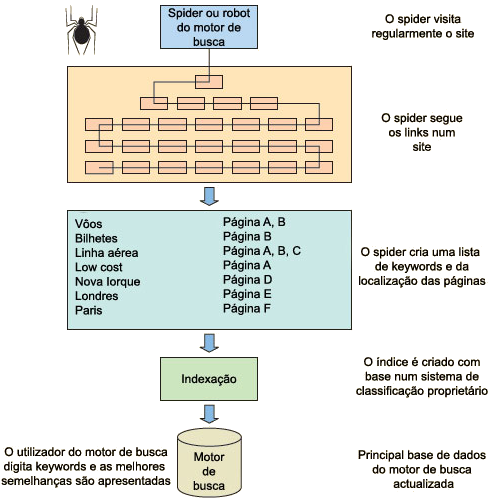
\includegraphics[width=60mm, height=60mm]{Figuras/BigData/Motordebusca.png}
\end{figure}

A utilização desses robôs é uma alternativa eficiente para coletar informações no Big data uma vez que essa é sua especialidade. 
Como o Big data tem uma forte componente de inconsistência, coletar informações das páginas visitas pelos robôs ou mesmo coletar a página inteira, pode ser 
extremamente eficiente nos quesitos ``volume'' e ``velocidade'' descrito na seção 2.3.2 (Hadoop -- Map Reduce -- Big Data). 


\section{Machine Learning}\label{arte:palavraChave:Machine}

O desafio dos 3 V's (Velocidade, Variedade e Volume) pode ser um fator determinístico na escolha da ferramenta mais adequada para analisar dados do \textit{Big Data} 
e extrair informação. As árvores de decisão são algoritmos rápidos, contudo dados impuros podem comprometer o desempenho desse algoritmo. A fase de extração dos dados do 
\textit{Big Data} é fortemente influenciáveis pelas variáveis escolhidas, \cite{DecisionTree} isso pode representar o desafio maior para implementar esta técnica. 
%na figura a seguir exemplificamos essa tarefa:


\subsection{Árvore de Decisão}

Han e Kamber \cite{DataMining} definem indução por árvore de decisão como a aprendizagem de árvore de decisão a partir de classes rotuladas nas tuplas de treinamento. 
A estrutura da árvore de decisão é semelhante a um fluxograma, onde cada nó interno (não-folha) indica um teste de atributo, cada ramo representa o resultado de um teste e 
cada nó da folha possui um rótulo de classe. O nó de nível mais superior é chamado de nó-raiz.
A seguir, a árvore de decisão que explicita se um cliente, de acodo com sua idade, irá efeturar ou não a compra de um computador:

\begin{figure}[!ht]
\centering
\caption{Árvore de decisão}
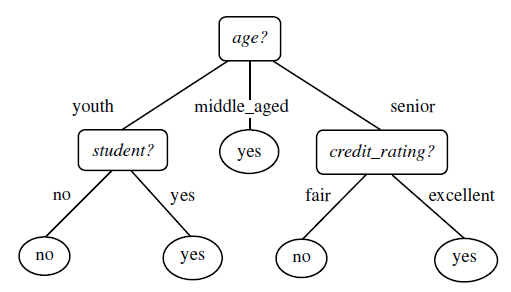
\includegraphics[width=60mm, height=40mm]{Figuras/BigData/arvore.png}
\end{figure}

Para Ian e Frank \cite{MachineLearning}, as árvores de decisão podem ser representadas por uma abordagem ``dividir para conquistar'' para resolução de problemas de 
aprendizagem, a partir de um conjunto de instâncias independentes. Os nós em uma árvore de decisão ``testam'' um atributo específico, comparando seu valor com uma constante.
No entanto, algumas árvores podem comparar dois atributos com outros ou utilizarem uma função para tal.
As árvores de decisão podem ser classificadas em dois tipos: árvores de regressão (regression trees), que são utilizadas para estimar atributos numéricos, e árvores de 
classificação (classification trees), usadas para análise de variáveis categóricas.

O algorítimo \textit{C4.5} é considerado um exemplo clássico de método de indução de árvores de decisão. O \textit{C4.5} \cite{Learning2007} foi inspirado no algoritmo 
\textit{ID3} \cite{Learning1979}, que produz árvores de decisão a partir de uma abordagem recursiva de particionamento de um conjunto de dados, utilizando conceitos e medidas 
da Teoria da Informação \cite{TeoriaInf}.

As árvores de decisão têm uma característica peculiar, a saída do modelo de predição (o output), com regras se -- então é claramente perceptivel por analistas humanos.
Essa qualidade é utilizada para interpretar os resultados.


\section{Regressão Logística}

Os modelos de regressão (linear e logística) são técnicas para analisar o relacionamento entre variáveis. No entanto, a regressão linear é utilizada para problemas de natureza
contínua, sendo que a regressão logística é semelhante, contudo, a variável dependente não é contínua, é discreta ou categórica \cite{DecisaoCredito}.

A regressão logística está definida como o logarítmo a seguir:

\begin{equation}
 log{\frac{\pi(x)}{1-\pi(x)}} = \beta_0 + \beta_1 x_1 + \beta_2 x_2 + ... + \beta_p x_p
\end{equation}

onde $\pi(x)$ é definido como:

\begin{equation}
 \pi(x) = \dfrac{1}{1 + e^{-{\beta_0 + \beta_1 x_1 + \beta_2 x_2 + ... + \beta_p x_p}}}
\end{equation}

e $x_1, x_2,..., x_p$ são as variáveis a serem exploradas.


A aplicação da regressão logística foi utilizada, pela primeira vez, com sucesso na oferta de crédito nos anos seguintes ao fim da 2ª guerra mundial, para tomar decisão 
de oferecer crédito a terceiros \cite{RegrecaoLog}.
A regressão logística é comumente aplicada para problemas de classificação binária (ou booleano).
